%
% new Latex2E GJI class file
% don't use "times" package because of a bug
\documentclass[onecolumn,extra]{gji_modified_cours_UPPA}
%
% T1 encoding gives better PDF and allows for 8 bits
\usepackage[T1]{fontenc}
\usepackage{times}
\usepackage{graphicx}
%
%%%%%%%%%%%%%%%%%%%%%%%%%%%%
%% A4 paper
%%%%%%%%%%%%%%%%%%%%%%%%%%%%
\textwidth 17cm
\textheight 24.8cm
\oddsidemargin -4.5mm
\evensidemargin -4.5mm
\topmargin -11mm

% biblio GJI
\bibliographystyle{gji}
\renewcommand{\cite}[1]{\citet{#1}}
% roman d for dV in integrals
\newcommand{\rmd}{\mathrm{d}}

% roman i for complex number
\newcommand{\myiomega}{\mathrm{i} \omega}

%bold lowercase roman letters

\newcommand{\ba}{\mbox{${\bf a}$}}
\newcommand{\bb}{\mbox{${\bf b}$}}
\newcommand{\bc}{\mbox{${\bf c}$}}
\newcommand{\bd}{\mbox{${\bf d}$}}
\newcommand{\be}{\mbox{${\bf e}$}}
\newcommand{\bef}{\mbox{${\bf f}$}}
\newcommand{\bg}{\mbox{${\bf g}$}}
\newcommand{\bh}{\mbox{${\bf h}$}}
\newcommand{\bi}{\mbox{${\bf i}$}}
\newcommand{\bj}{\mbox{${\bf j}$}}
\newcommand{\bk}{\mbox{${\bf k}$}}
\newcommand{\bl}{\mbox{${\bf l}$}}
\newcommand{\bm}{\mbox{${\bf m}$}}
\newcommand{\bn}{\mbox{${\bf n}$}}
\newcommand{\bo}{\mbox{${\bf o}$}}
\newcommand{\bp}{\mbox{${\bf p}$}}
\newcommand{\bq}{\mbox{${\bf q}$}}
\newcommand{\br}{\mbox{${\bf r}$}}
\newcommand{\bs}{\mbox{${\bf s}$}}
\newcommand{\bt}{\mbox{${\bf t}$}}
\newcommand{\bu}{\mbox{${\bf u}$}}
\newcommand{\bv}{\mbox{${\bf v}$}}
\newcommand{\bw}{\mbox{${\bf w}$}}
\newcommand{\bx}{\mbox{${\bf x}$}}
\newcommand{\by}{\mbox{${\bf y}$}}
\newcommand{\bz}{\mbox{${\bf z}$}}

%bold uppercase roman letters

\newcommand{\bA}{\mbox{${\bf A}$}}
\newcommand{\bB}{\mbox{${\bf B}$}}
\newcommand{\bC}{\mbox{${\bf C}$}}
\newcommand{\bD}{\mbox{${\bf D}$}}
\newcommand{\bE}{\mbox{${\bf E}$}}
\newcommand{\bF}{\mbox{${\bf F}$}}
\newcommand{\bG}{\mbox{${\bf G}$}}
\newcommand{\bH}{\mbox{${\bf H}$}}
\newcommand{\bI}{\mbox{${\bf I}$}}
\newcommand{\bJ}{\mbox{${\bf J}$}}
\newcommand{\bK}{\mbox{${\bf K}$}}
\newcommand{\bL}{\mbox{${\bf L}$}}
\newcommand{\bM}{\mbox{${\bf M}$}}
\newcommand{\bN}{\mbox{${\bf N}$}}
\newcommand{\bO}{\mbox{${\bf O}$}}
\newcommand{\bP}{\mbox{${\bf P}$}}
\newcommand{\bQ}{\mbox{${\bf Q}$}}
\newcommand{\bR}{\mbox{${\bf R}$}}
\newcommand{\bS}{\mbox{${\bf S}$}}
\newcommand{\bT}{\mbox{${\bf T}$}}
\newcommand{\bU}{\mbox{${\bf U}$}}
\newcommand{\bV}{\mbox{${\bf V}$}}
\newcommand{\bW}{\mbox{${\bf W}$}}
\newcommand{\bX}{\mbox{${\bf X}$}}
\newcommand{\bY}{\mbox{${\bf Y}$}}
\newcommand{\bZ}{\mbox{${\bf Z}$}}

%script upper case letters

\newcommand{\sA}{\mbox{$\cal A$}}
\newcommand{\sB}{\mbox{$\cal B$}}
\newcommand{\sC}{\mbox{$\cal C$}}
\newcommand{\sD}{\mbox{$\cal D$}}
\newcommand{\sE}{\mbox{$\cal E$}}
\newcommand{\sF}{\mbox{$\cal F$}}
\newcommand{\sG}{\mbox{$\cal G$}}
\newcommand{\sH}{\mbox{$\cal H$}}
\newcommand{\sI}{\mbox{$\cal I$}}
\newcommand{\sJ}{\mbox{$\cal J$}}
\newcommand{\sK}{\mbox{$\cal K$}}
\newcommand{\sL}{\mbox{$\cal L$}}
\newcommand{\sM}{\mbox{$\cal M$}}
\newcommand{\sN}{\mbox{$\cal N$}}
\newcommand{\sO}{\mbox{$\cal O$}}
\newcommand{\sP}{\mbox{$\cal P$}}
\newcommand{\sQ}{\mbox{$\cal Q$}}
\newcommand{\sR}{\mbox{$\cal R$}}
\newcommand{\sS}{\mbox{$\cal S$}}
\newcommand{\sT}{\mbox{$\cal T$}}
\newcommand{\sU}{\mbox{$\cal U$}}
\newcommand{\sV}{\mbox{$\cal V$}}
\newcommand{\sW}{\mbox{$\cal W$}}
\newcommand{\sX}{\mbox{$\cal X$}}
\newcommand{\sY}{\mbox{$\cal Y$}}
\newcommand{\sZ}{\mbox{$\cal Z$}}

%bold upper case script letters

\newcommand{\bsA}{\mbox{\boldmath$\cal A$}}
\newcommand{\bsB}{\mbox{\boldmath$\cal B$}}
\newcommand{\bsC}{\mbox{\boldmath$\cal C$}}
\newcommand{\bsD}{\mbox{\boldmath$\cal D$}}
\newcommand{\bsE}{\mbox{\boldmath$\cal E$}}
\newcommand{\bsF}{\mbox{\boldmath$\cal F$}}
\newcommand{\bsG}{\mbox{\boldmath$\cal G$}}
\newcommand{\bsH}{\mbox{\boldmath$\cal H$}}
\newcommand{\bsI}{\mbox{\boldmath$\cal I$}}
\newcommand{\bsJ}{\mbox{\boldmath$\cal J$}}
\newcommand{\bsK}{\mbox{\boldmath$\cal K$}}
\newcommand{\bsL}{\mbox{\boldmath$\cal L$}}
\newcommand{\bsM}{\mbox{\boldmath$\cal M$}}
\newcommand{\bsN}{\mbox{\boldmath$\cal N$}}
\newcommand{\bsO}{\mbox{\boldmath$\cal O$}}
\newcommand{\bsP}{\mbox{\boldmath$\cal P$}}
\newcommand{\bsQ}{\mbox{\boldmath$\cal Q$}}
\newcommand{\bsR}{\mbox{\boldmath$\cal R$}}
\newcommand{\bsS}{\mbox{\boldmath$\cal S$}}
\newcommand{\bsT}{\mbox{\boldmath$\cal T$}}
\newcommand{\bsU}{\mbox{\boldmath$\cal U$}}
\newcommand{\bsV}{\mbox{\boldmath$\cal V$}}
\newcommand{\bsW}{\mbox{\boldmath$\cal W$}}
\newcommand{\bsX}{\mbox{\boldmath$\cal X$}}
\newcommand{\bsY}{\mbox{\boldmath$\cal Y$}}
\newcommand{\bsZ}{\mbox{\boldmath$\cal Z$}}

%upper case sans serif letters

\newcommand{\ssA}{\mbox{${\sf A}$}}
\newcommand{\ssB}{\mbox{${\sf B}$}}
\newcommand{\ssC}{\mbox{${\sf C}$}}
\newcommand{\ssD}{\mbox{${\sf D}$}}
\newcommand{\ssE}{\mbox{${\sf E}$}}
\newcommand{\ssF}{\mbox{${\sf F}$}}
\newcommand{\ssG}{\mbox{${\sf G}$}}
\newcommand{\ssH}{\mbox{${\sf H}$}}
\newcommand{\ssI}{\mbox{${\sf I}$}}
\newcommand{\ssJ}{\mbox{${\sf J}$}}
\newcommand{\ssK}{\mbox{${\sf K}$}}
\newcommand{\ssL}{\mbox{${\sf L}$}}
\newcommand{\ssM}{\mbox{${\sf M}$}}
\newcommand{\ssN}{\mbox{${\sf N}$}}
\newcommand{\ssO}{\mbox{${\sf O}$}}
\newcommand{\ssP}{\mbox{${\sf P}$}}
\newcommand{\ssQ}{\mbox{${\sf Q}$}}
\newcommand{\ssR}{\mbox{${\sf R}$}}
\newcommand{\ssS}{\mbox{${\sf S}$}}
\newcommand{\ssT}{\mbox{${\sf T}$}}
\newcommand{\ssU}{\mbox{${\sf U}$}}
\newcommand{\ssV}{\mbox{${\sf V}$}}
\newcommand{\ssW}{\mbox{${\sf W}$}}
\newcommand{\ssX}{\mbox{${\sf X}$}}
\newcommand{\ssY}{\mbox{${\sf Y}$}}
\newcommand{\ssZ}{\mbox{${\sf Z}$}}

%lower case sans serif letters

\newcommand{\ssa}{\mbox{${\sf a}$}}
\newcommand{\ssb}{\mbox{${\sf b}$}}
\newcommand{\ssc}{\mbox{${\sf c}$}}
\newcommand{\ssd}{\mbox{${\sf d}$}}
\newcommand{\sse}{\mbox{${\sf e}$}}
\newcommand{\ssf}{\mbox{${\sf f}$}}
\newcommand{\ssg}{\mbox{${\sf g}$}}
\newcommand{\ssh}{\mbox{${\sf h}$}}
\newcommand{\ssi}{\mbox{${\sf i}$}}
\newcommand{\ssj}{\mbox{${\sf j}$}}
\newcommand{\ssk}{\mbox{${\sf k}$}}
\newcommand{\ssl}{\mbox{${\sf l}$}}
\newcommand{\ssm}{\mbox{${\sf m}$}}
\newcommand{\ssn}{\mbox{${\sf n}$}}
\newcommand{\sso}{\mbox{${\sf o}$}}
\newcommand{\ssp}{\mbox{${\sf p}$}}
\newcommand{\ssq}{\mbox{${\sf q}$}}
\newcommand{\ssr}{\mbox{${\sf r}$}}
\newcommand{\sss}{\mbox{${\sf s}$}}
\newcommand{\sst}{\mbox{${\sf t}$}}
\newcommand{\ssu}{\mbox{${\sf u}$}}
\newcommand{\ssv}{\mbox{${\sf v}$}}
\newcommand{\ssw}{\mbox{${\sf w}$}}
\newcommand{\ssx}{\mbox{${\sf x}$}}
\newcommand{\ssy}{\mbox{${\sf y}$}}
\newcommand{\ssz}{\mbox{${\sf z}$}}

%bold lowercase greek letters

\newcommand{\balpha}{\mbox{\boldmath $\bf \alpha$}}
\newcommand{\bbeta}{\mbox{\boldmath $\bf \beta$}}
\newcommand{\bgamma}{\mbox{\boldmath $\bf \gamma$}}
\newcommand{\bdelta}{\mbox{\boldmath $\bf \delta$}}
\newcommand{\bepsilon}{\mbox{\boldmath $\bf \varepsilon$}}
\newcommand{\beps}{\mbox{\boldmath $\bf \varepsilon$}}
\newcommand{\bzeta}{\mbox{\boldmath $\bf \zeta$}}
\newcommand{\boeta}{\mbox{\boldmath $\bf \eta$}}
\newcommand{\btheta}{\mbox{\boldmath $\bf \theta$}}
\newcommand{\bkappa}{\mbox{\boldmath $\bf \kappa$}}
\newcommand{\blambda}{\mbox{\boldmath $\bf \lambda$}}
\newcommand{\bmu}{\mbox{\boldmath $\bf \mu$}}
\newcommand{\bnu}{\mbox{\boldmath $\bf \nu$}}
\newcommand{\bxi}{\mbox{\boldmath $\bf \xi$}}
\newcommand{\bpi}{\mbox{\boldmath $\bf \pi$}}
\newcommand{\bsigma}{\mbox{\boldmath $\bf \sigma$}}
\newcommand{\btau}{\mbox{\boldmath $\bf \tau$}}
\newcommand{\bupsilon}{\mbox{\boldmath $\bf \upsilon$}}
\newcommand{\bphi}{\mbox{\boldmath $\bf \phi$}}
\newcommand{\bchi}{\mbox{\boldmath $\bf \chi$}}
\newcommand{\bpsi}{\mbox{\boldmath$ \bf \psi$}}
\newcommand{\bomega}{\mbox{\boldmath $\bf \omega$}}
\newcommand{\bom}{\mbox{\boldmath $\bf \omega$}}

%bold uppercase greek letters

\newcommand{\bGamma}{\mbox{\boldmath $\bf \Gamma$}}
\newcommand{\bDelta}{\mbox{\boldmath $\bf \Delta$}}
\newcommand{\bLambda}{\mbox{\boldmath $\bf \Lambda$}}
\newcommand{\bXi}{\mbox{\boldmath $\bf \Xi$}}
\newcommand{\bPi}{\mbox{\boldmath $\bf \Pi$}}
\newcommand{\bSigma}{\mbox{\boldmath $\bf \Sigma$}}
\newcommand{\bUpsilon}{\mbox{\boldmath $\bf \Upsilon$}}
\newcommand{\bPhi}{\mbox{\boldmath $\bf \Phi$}}
\newcommand{\bPsi}{\mbox{\boldmath $\bf \Psi$}}
\newcommand{\bOmega}{\mbox{\boldmath $\bf \Omega$}}
\newcommand{\bOm}{\mbox{\boldmath $\bf \Omega$}}

%sans serif greek letters and numbers

\newcommand{\ssDelta}{\mbox{${\sf \Delta}$}}
\newcommand{\ssLambda}{\mbox{${\sf \Lambda}$}}
\newcommand{\ssGamma}{\mbox{${\sf \Gamma}$}}
\newcommand{\ssOmega}{\mbox{${\sf \Omega}$}}
\newcommand{\ssSigma}{\mbox{${\sf \Sigma}$}}
\newcommand{\sszero}{\mbox{${\sf 0}$}}

%bold unit vectors

\newcommand{\bCh}{\mbox{$\hat{\mbox{${\bf C}$}}$}}
\newcommand{\bGh}{\mbox{$\hat{\mbox{${\bf G}$}}$}}
\newcommand{\bah}{\mbox{$\hat{\mbox{${\bf a}$}}$}}
\newcommand{\bbh}{\mbox{$\hat{\mbox{${\bf b}$}}$}}
\newcommand{\beh}{\mbox{$\hat{\mbox{${\bf e}$}}$}}
\newcommand{\bgh}{\mbox{$\hat{\mbox{${\bf g}$}}$}}
\newcommand{\bkh}{\mbox{$\hat{\mbox{${\bf k}$}}$}}
\newcommand{\bnh}{\mbox{$\hat{\mbox{${\bf n}$}}$}}
\newcommand{\bph}{\mbox{$\hat{\mbox{${\bf p}$}}$}}
\newcommand{\brh}{\mbox{$\hat{\mbox{${\bf r}$}}$}}
\newcommand{\bth}{\mbox{$\hat{\mbox{${\bf t}$}}$}}
\newcommand{\bxh}{\mbox{$\hat{\mbox{${\bf x}$}}$}}
\newcommand{\byh}{\mbox{$\hat{\mbox{${\bf y}$}}$}}
\newcommand{\bzh}{\mbox{$\hat{\mbox{${\bf z}$}}$}}
\newcommand{\bnuh}{\mbox{$\hat{\mbox{\boldmath $\bf \nu$}}$}}
\newcommand{\betah}{\mbox{$\hat{\mbox{\boldmath $\bf \eta$}}$}}
\newcommand{\bthetah}{\mbox{$\hat{\mbox{\boldmath $\bf \theta$}}$}}
\newcommand{\bphih}{\mbox{$\hat{\mbox{\boldmath $\bf \phi$}}$}}
\newcommand{\bDeltah}{\mbox{$\hat{\mbox{\boldmath $\bf \Delta$}}$}}
\newcommand{\bThetah}{\mbox{$\hat{\mbox{\boldmath $\bf \Theta$}}$}}
\newcommand{\bPhih}{\mbox{$\hat{\mbox{\boldmath $\bf \Phi$}}$}}
\newcommand{\bsigmah}{\mbox{$\hat{\mbox{\boldmath $\bf \sigma$}}$}}
\newcommand{\bthetahpr}{\mbox{$\hat{\mbox{\boldmath $\bf \theta$}}
            ^{\raise-.5ex\hbox{$\scriptstyle\prime$}}$}}
\newcommand{\bphihpr}{\mbox{$\hat{\mbox{\boldmath $\bf \phi$}}
            ^{\raise-.5ex\hbox{$\scriptstyle\prime$}}$}}
\newcommand{\bThetahpr}{\mbox{$\hat{\mbox{\boldmath $\bf \Theta$}}
            ^{\raise-.5ex\hbox{$\scriptstyle\prime$}}$}}
\newcommand{\bPhihpr}{\mbox{$\hat{\mbox{\boldmath $\bf \Phi$}}
            ^{\raise-.5ex\hbox{$\scriptstyle\prime$}}$}}

%subscripts

\newcommand{\spar}{\mbox{$\scriptstyle\partial$}}
\newcommand{\sbdel}{\mbox{\boldmath $\scriptstyle\nabla$}}
\newcommand{\subk}{\mbox{\scriptsize\bf k}}
\newcommand{\subp}{\mbox{\scriptsize\bf p}}
\newcommand{\subr}{\mbox{\scriptsize\bf r}}
\newcommand{\subs}{\mbox{\scriptsize\bf s}}
\newcommand{\subx}{\mbox{\scriptsize\bf x}}
\newcommand{\subxi}{\mbox{$\scriptstyle{\bf \xi}$}}
\newcommand{\subrho}{\mbox{$\scriptstyle\rho$}}
\newcommand{\subphi}{\mbox{$\scriptstyle\phi$}}
\newcommand{\subpsi}{\mbox{$\scriptstyle\psi$}}
\newcommand{\subnhat}{\mbox{\scriptsize{$\hat{\mbox{${\bf n}$}}$}}}
\newcommand{\subearth}{\raise.15ex\hbox{$\scriptstyle\oplus$}}
\newcommand{\subhalf}{\mbox{$\scriptstyle\frac{1}{2}$}}
\newcommand{\subspace}{\raise.25ex\hbox{$\scriptscriptstyle\bigcirc$}}

%fractions

\newcommand{\half}{\mbox{$\frac{1}{2}$}}
\newcommand{\third}{\mbox{$\frac{1}{3}$}}
\newcommand{\fifth}{\mbox{$\frac{1}{5}$}}
\newcommand{\fourth}{\mbox{$\frac{1}{4}$}}
% DK DK for GJI style file \newcommand{\twothirds}{\mbox{$\frac{2}{3}$}}
\newcommand{\fourthirds}{\mbox{$\frac{4}{3}$}}
\newcommand{\threehalves}{\mbox{$\frac{3}{2}$}}
\newcommand{\fivehalves}{\mbox{$\frac{5}{2}$}}
\newcommand{\threefourths}{\mbox{$\frac{3}{4}$}}
\newcommand{\threeeighths}{\mbox{$\frac{3}{8}$}}
\newcommand{\fivesixteenths}{\mbox{$\frac{5}{16}$}}
\newcommand{\fivefourths}{\mbox{$\frac{5}{4}$}}
\newcommand{\ninefourths}{\mbox{$\frac{9}{4}$}}
\newcommand{\threefifths}{\mbox{$\frac{3}{5}$}}
\newcommand{\fivethirds}{\mbox{$\frac{5}{3}$}}
\newcommand{\eightthirds}{\mbox{$\frac{8}{3}$}}
\newcommand{\fourninths}{\mbox{$\frac{4}{9}$}}
\newcommand{\fiveninths}{\mbox{$\frac{5}{9}$}}
\newcommand{\sixteenthirds}{\mbox{$\frac{16}{3}$}}
\newcommand{\sixteenninths}{\mbox{$\frac{16}{9}$}}
\newcommand{\nineteenhalves}{\mbox{$\frac{19}{2}$}}
\newcommand{\quart}{\mbox{$\frac{1}{4}$}}
\newcommand{\eighth}{\mbox{$\frac{1}{8}$}}
\newcommand{\ninth}{\mbox{$\frac{1}{9}$}}
\newcommand{\tenth}{\mbox{$\frac{1}{10}$}}
\newcommand{\fifteenth}{\mbox{$\frac{1}{15}$}}
\newcommand{\sixth}{\mbox{$\frac{1}{6}$}}
\newcommand{\seventhirds}{\mbox{$\frac{7}{3}$}}
\newcommand{\invpi}{\mbox{$\frac{1}{\pi}$}}
\newcommand{\twoinvpi}{\mbox{$\frac{2}{\pi}$}}
\newcommand{\invtwopi}{\mbox{$\frac{1}{2\pi}$}}

%other miscellaneous definitions

\newcommand{\om}{\mbox{$\omega$}}
\newcommand{\Om}{\mbox{$\Omega$}}
\newcommand{\ep}{\mbox{$\varepsilon$}}
% DK DK for GJI style file \newcommand{\eps}{\mbox{$\varepsilon$}}
\newcommand{\p}{\mbox{$\partial$}}
\newcommand{\del}{\mbox{$\nabla$}}
\newcommand{\bdel}{\mbox{\boldmath $\nabla$}}
\newcommand{\bzero}{\mbox{${\bf 0}$}}
\renewcommand{\Re}{\mbox{${\rm R}$}}
\renewcommand{\Im}{\mbox{${\rm I}$}}
\newcommand{\real}{\mbox{$\Re{\rm e}$}}
\newcommand{\imag}{\mbox{$\Im{\rm m}$}}
\newcommand{\sqL}{\mbox{$k$}}
\newcommand{\sqLinv}{\mbox{$k^{-1}$}}
\newcommand{\nunl}{\mbox{${}_n\nu_l$}}
% DK DK for GJI style file \newcommand{\earth}{\raise.15ex\hbox{$\oplus$}}
\newcommand{\tdot}{\,.\hspace{-0.98 mm}\raise.6ex\hbox{.}
                   \hspace{-0.98 mm}\raise1.2ex\hbox{.}\,}
\newcommand{\pvint}{\mathbin{\int{\mkern-19.2mu}-}}
\newcommand{\allspace}{\raise.25ex\hbox{$\scriptstyle\bigcirc$}}

%miscellaneous definitions jeroen paris visit

\newcommand{\bTt}{\mbox{$\widetilde{{\bf T}}$}}
\newcommand{\ylm}{\mbox{${\cal Y}_{lm}$}}
\newcommand{\Un}{\mbox{$U_n$}}
\newcommand{\Vn}{\mbox{$V_n$}}
\newcommand{\Fn}{\mbox{$F_n$}}
\newcommand{\Hn}{\mbox{$H_n$}}
\newcommand{\Pn}{\mbox{$P_n$}}
\newcommand{\Wn}{\mbox{$W_n$}}
\newcommand{\Gn}{\mbox{$G_n$}}
\newcommand{\an}{\mbox{$a_n$}}
\newcommand{\kn}{\mbox{$k_n$}}
\newcommand{\omn}{\mbox{$\omega_n$}}
\newcommand{\alphan}{\mbox{$\alpha_n$}}
\newcommand{\Unl}{\mbox{${}_nU_l$}}
\newcommand{\sUnl}{\mbox{${}_{n\hspace{0.2 mm}}\sU_l$}}
\newcommand{\sVnl}{\mbox{${}_{n\hspace{-0.4 mm}}\sV_l$}}
\newcommand{\sWnl}{\mbox{${}_{n\hspace{-0.3 mm}}\sW_l$}}
\newcommand{\sPnl}{\mbox{${}_n\sP_l$}}
\newcommand{\Fnl}{\mbox{${}_nF_l$}}
\newcommand{\Gnl}{\mbox{${}_nG_l$}}
\newcommand{\Anl}{\mbox{${}_nA_l$}}
\newcommand{\Hnl}{\mbox{${}_nH_l$}}
\newcommand{\Vnl}{\mbox{${}_nV_l$}}
\newcommand{\Wnl}{\mbox{${}_nW_l$}}
\newcommand{\Pnl}{\mbox{${}_nP_l$}}
\newcommand{\Rnl}{\mbox{${}_nR_l$}}
\newcommand{\Snl}{\mbox{${}_nS_l$}}
\newcommand{\Tnl}{\mbox{${}_nT_l$}}
\newcommand{\Knl}{\mbox{${}_nK_l$}}
\newcommand{\bAnlm}{\mbox{${}_n\bA_{lm}$}}
\newcommand{\bBnlm}{\mbox{${}_n\bB_{lm}$}}
\newcommand{\bAnm}{\mbox{${}_n\bA_{m}$}}
\newcommand{\bBnm}{\mbox{${}_n\bB_{m}$}}
\newcommand{\bGnm}{\mbox{${}_n\bG_{m}$}}
\newcommand{\bRnl}{\mbox{${}_n\bR_l$}}
\newcommand{\bDnl}{\mbox{${}_n\bD_l$}}
\newcommand{\bsDnl}{\mbox{${}_{n\hspace{-0.2 mm}}\bsD_l$}}
\newcommand{\bEnl}{\mbox{${}_n\bE_l$}}
\newcommand{\bsEnl}{\mbox{${}_n\bsE_l$}}
\newcommand{\bTnlm}{\mbox{${}_n\bT_{lm}$}}
\newcommand{\bsnlm}{\mbox{${}_n\bs_{lm}$}}
\newcommand{\phinlm}{\mbox{${}_n\phi_{lm}$}}
\newcommand{\dUnl}{\mbox{${}_n\dot{U}_l$}}
\newcommand{\dVnl}{\mbox{${}_n\dot{V}_l$}}
\newcommand{\dWnl}{\mbox{${}_n\dot{W}_l$}}
\newcommand{\dPnl}{\mbox{${}_n\dot{P}_l$}}
\newcommand{\Unlm}{\mbox{${}_nU_{lm}$}}
\newcommand{\Vnlm}{\mbox{${}_nV_{lm}$}}
\newcommand{\Wnlm}{\mbox{${}_nW_{lm}$}}
\newcommand{\Rnlm}{\mbox{${}_nR_{lm}$}}
\newcommand{\Snlm}{\mbox{${}_nS_{lm}$}}
\newcommand{\Tnlm}{\mbox{${}_nT_{lm}$}}
\newcommand{\Pnlm}{\mbox{${}_nP_{lm}$}}
\newcommand{\dRnl}{\mbox{${}_n\dot{R}_l$}}
\newcommand{\dSnl}{\mbox{${}_n\dot{S}_l$}}
\newcommand{\dTnl}{\mbox{${}_n\dot{T}_l$}}
\newcommand{\dKnl}{\mbox{${}_n\dot{K}_l$}}
\newcommand{\omnl}{\mbox{${}_{n\hspace{-0.2 mm}}\omega_l$}}
\newcommand{\gammanl}{\mbox{${}_{n\hspace{-0.5 mm}}\gamma_l$}}
\newcommand{\omnlm}{\mbox{${}_n\omega_{lm}$}}
\newcommand{\dU}{\mbox{$\dot{U}$}}
\newcommand{\dV}{\mbox{$\dot{V}$}}
\newcommand{\dW}{\mbox{$\dot{W}$}}
\newcommand{\dP}{\mbox{$\dot{P}$}}
\newcommand{\dR}{\mbox{$\dot{R}$}}
\newcommand{\dS}{\mbox{$\dot{S}$}}
\newcommand{\dT}{\mbox{$\dot{T}$}}
\newcommand{\dK}{\mbox{$\dot{K}$}}
\newcommand{\dsU}{\mbox{$\dot{\sU}$}}
\newcommand{\dsV}{\mbox{$\dot{\sV}$}}
\newcommand{\dsW}{\mbox{$\dot{\sW}$}}
\newcommand{\dsP}{\mbox{$\dot{\sP}$}}
\newcommand{\dg}{\mbox{$\dot{g}$}}
\newcommand{\dy}{\mbox{$\dot{y}$}}
\newcommand{\ddy}{\mbox{$\ddot{y}$}}
\newcommand{\dr}{\mbox{$\dot{r}$}}
\newcommand{\dearth}{\mbox{$\dot{\earth}$}}
\newcommand{\dpp}{\mbox{$\dot{p}$}}
\newcommand{\ds}{\mbox{$\dot{s}$}}
\newcommand{\dphi}{\mbox{$\dot{\phi}$}}
\newcommand{\dkappa}{\mbox{$\dot{\kappa}$}}
\newcommand{\dmu}{\mbox{$\dot{\mu}$}}
\newcommand{\drho}{\mbox{$\dot{\rho}$}}
\newcommand{\dPhi}{\mbox{$\dot{\Phi}$}}
\newcommand{\ddU}{\mbox{$\ddot{U}$}}
\newcommand{\ddV}{\mbox{$\ddot{V}$}}
\newcommand{\ddW}{\mbox{$\ddot{W}$}}
\newcommand{\ddP}{\mbox{$\ddot{P}$}}
\newcommand{\ddphi}{\mbox{$\ddot{\phi}$}}
\newcommand{\ddPhi}{\mbox{$\ddot{\Phi}$}}

%miscellaneous definitions jeroen appendix D

\newcommand{\uu}{\mbox{$u$}}
\newcommand{\du}{\mbox{$\dot{u}$}}
\newcommand{\vv}{\mbox{$v$}}
\newcommand{\dv}{\mbox{$\dot{v}$}}
\newcommand{\w}{\mbox{$w$}}
\newcommand{\dw}{\mbox{$\dot{w}$}}
\newcommand{\ph}{\mbox{$p$}}
\newcommand{\dph}{\mbox{$\dot{p}$}}
\newcommand{\f}{\mbox{$f$}}
\newcommand{\x}{\mbox{$x$}}
\newcommand{\z}{\mbox{$z$}}
\newcommand{\el}{\mbox{$k^2$}}
%%%%%%%%\newcommand{\up}{\mbox{$u'$}}
\newcommand{\dup}{\mbox{$\dot{u}'$}}
\newcommand{\vp}{\mbox{$v'$}}
\newcommand{\dvp}{\mbox{$\dot{v}'$}}
\newcommand{\wwp}{\mbox{$w'$}}
\newcommand{\dwp}{\mbox{$\dot{w}'$}}
\newcommand{\php}{\mbox{$p'$}}
\newcommand{\dphp}{\mbox{$\dot{p}'$}}
% DK DK for GJI style file \newcommand{\fp}{\mbox{$f'$}}
\newcommand{\xp}{\mbox{$x'$}}
\newcommand{\zp}{\mbox{$z'$}}
\newcommand{\lp}{\mbox{$k'^2$}}

%miscellaneous definitions jeroen chapter 14

\newcommand{\dombar}{\mbox{$\delta\bar{\omega}$}}
\newcommand{\otheta}{{\bar{\theta}}}
\newcommand{\ophi}{{\bar{\phi}}}
\newcommand{\eightfifteenths}{\mbox{$\frac{8}{15}$}}
\newcommand{\twentyfivefourths}{\mbox{$\frac{25}{4}$}}
\newcommand{\twofifteenth}{\mbox{$\frac{2}{15}$}}

%equation formatting

\newcommand{\eq}{\begin{equation}}
\newcommand{\en}{\end{equation}}
\newcommand{\eqa}{\begin{eqnarray}}
\newcommand{\ena}{\end{eqnarray}}

%fattened bold Greek subscripts

\newcommand{\subtau}{\mbox{\boldmath $\scriptstyle{\tau}$}}
\newcommand{\subLambda}{\mbox{\boldmath $\scriptstyle{\Lambda}$}}
\newcommand{\subGamma}{\mbox{\boldmath $\scriptstyle{\Gamma}$}}

%sans serif lower case delta and eta

\newcommand{\grss}{\fontencoding{LGR}\fontfamily{cmss}\selectfont}
\newcommand{\ssdelta}{\mbox{\grss d}}
\newcommand{\sseta}{\mbox{\grss h}}


\begin{document}

\title{Notes about 3D C-PML equations for SPECFEM3D}
%
\author[Dimitri Komatitsch, Zhinan Xie]{Dimitri Komatitsch, Zhinan Xie\\
CNRS Marseille, France}
%
\date{September 22, 2012}

\maketitle

\begin{figure}
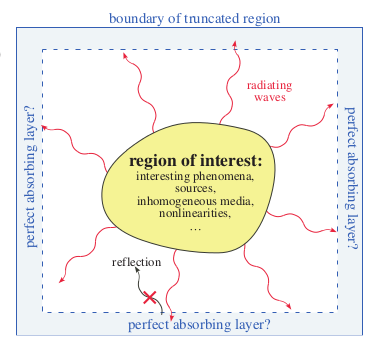
\includegraphics[scale=0.5]{pml_schematic.png}
\caption{Schematic of a typical wave-equation problem, in which there is some finite region of interest where sources,
inhomogeneous media, nonlinearities and etc are being investigated, from which some radiative waves escape to infinity.
The perfect absorbing layer, which was used to truncated out computational region, is placed adjacent to the edges of the
computational region}
\end{figure}

\noindent
Adjacent to 3DCPML, we assume the motion is governed by 3D elastic wave equation. In differential form it is given by:
%
\begin{eqnarray}
\varepsilon_{xx} & = & \partial_x u_x \nonumber \\
\varepsilon_{yy} & = & \partial_y u_y \nonumber \\
\varepsilon_{zz} & = & \partial_z u_z \nonumber \\
\varepsilon_{xy} & = & \frac{1}{2} (\partial_x u_y + \partial_y u_x) \,\, , \,\, \varepsilon_{yx} =  \varepsilon_{xy} \nonumber \\
\varepsilon_{xz} & = & \frac{1}{2} (\partial_x u_z + \partial_z u_x) \,\, , \,\, \varepsilon_{zx} =  \varepsilon_{xz} \nonumber \\
\varepsilon_{yz} & = & \frac{1}{2} (\partial_y u_z + \partial_z u_y) \,\, , \,\, \varepsilon_{zy} =  \varepsilon_{yz}
\end{eqnarray}
%
\noindent and
%
\begin{eqnarray}
\sigma_{xx} & = & (\lambda + 2 \mu) \, \varepsilon_{xx} + \lambda \, \varepsilon_{yy} + \lambda \, \varepsilon_{zz} \nonumber \\
\sigma_{yy} & = & \lambda \, \varepsilon_{xx} + (\lambda + 2 \mu) \, \varepsilon_{yy} + \lambda \, \varepsilon_{zz} \nonumber \\
\sigma_{zz} & = & \lambda \, \varepsilon_{xx} + \lambda \, \varepsilon_{yy} + (\lambda + 2 \mu) \, \varepsilon_{zz} \nonumber \\
\sigma_{xy} & = & 2 \mu \, \varepsilon_{xy} \,\, , \,\, \sigma_{yx} =  \sigma_{xy} \nonumber \\
\sigma_{xz} & = & 2 \mu \, \varepsilon_{xz} \,\, , \,\, \sigma_{zx} =  \sigma_{xz} \nonumber \\
\sigma_{yz} & = & 2 \mu \, \varepsilon_{yz} \,\, , \,\, \sigma_{yz} =  \sigma_{zy}
\end{eqnarray}
%
\noindent and
%
\begin{eqnarray}
\rho \, \frac{\partial^2 u_x}{\partial t^2} & = & \partial_x \sigma_{xx} + \partial_y \sigma_{xy} + \partial_z \sigma_{xz} + f_x \nonumber \\
\rho \, \frac{\partial^2 u_y}{\partial t^2} & = & \partial_x \sigma_{yx} + \partial_y \sigma_{yy} + \partial_z \sigma_{yz} + f_y \nonumber \\
\rho \, \frac{\partial^2 u_z}{\partial t^2} & = & \partial_x \sigma_{zx} + \partial_y \sigma_{zy} + \partial_z \sigma_{zz} + f_z
\end{eqnarray}

%%%%%%%%%%%%%%%%%%%%%%%%%%%%%%%%%%%%%%%%
%
\clearpage
%
%\noindent To obtain the CPML form, we just need to replace each spatial derivative with that same derivative multiplied by $1/s$.
%Thus, with CPML, in differential form in 2D this gives (noting $\frac{\partial^2 u_x}{\partial t^2}$ instead of $-\omega^2 u_x$ for now, even though we perform a Fourier transform,
%because we will perform an inverse Fourier transform later and thus get the term $\frac{\partial^2 u_x}{\partial t^2}$ back):
%
\noindent To obtain the CPML form, we firstly perform a Fourier transform on above equation,
then replace each spatial derivative with that same derivative multiplied by $1/s$
to make the plane wave entering into CPML without reflection and decaying exponentially along the x, y, z or in all directions.
Thus,in differential form in 3D the frequency-domain equation govened the motion in CPML gives:
%
\begin{eqnarray}
\varepsilon_{xx} & = & \frac{1}{s_x}\partial_x u_x \nonumber \\
\varepsilon_{yy} & = & \frac{1}{s_y}\partial_y u_y \nonumber \\
\varepsilon_{zz} & = & \frac{1}{s_z}\partial_z u_z \nonumber \\
\varepsilon_{xy} & = & \frac{1}{2} (\frac{1}{s_x} \partial_x u_y + \frac{1}{s_y} \partial_y u_x) \,\, , \,\, \varepsilon_{yx} =  \varepsilon_{xy} \nonumber \\
\varepsilon_{xz} & = & \frac{1}{2} (\frac{1}{s_x} \partial_x u_z + \frac{1}{s_z} \partial_z u_x) \,\, , \,\, \varepsilon_{zx} =  \varepsilon_{xz} \nonumber \\
\varepsilon_{yz} & = & \frac{1}{2} (\frac{1}{s_y} \partial_y u_z + \frac{1}{s_z} \partial_z u_y) \,\, , \,\, \varepsilon_{zy} =  \varepsilon_{yz}
\end{eqnarray}
%
\noindent and
%
\begin{eqnarray}
\sigma_{xx} & = & (\lambda + 2 \mu) \, \varepsilon_{xx} + \lambda \, \varepsilon_{yy} + \lambda \, \varepsilon_{zz} \nonumber \\
\sigma_{yy} & = & \lambda \, \varepsilon_{xx} + (\lambda + 2 \mu) \, \varepsilon_{yy} + \lambda \, \varepsilon_{zz} \nonumber \\
\sigma_{zz} & = & \lambda \, \varepsilon_{xx} + \lambda \, \varepsilon_{yy} + (\lambda + 2 \mu) \, \varepsilon_{zz} \nonumber \\
\sigma_{xy} & = & 2 \mu \, \varepsilon_{xy} \,\, , \,\, \sigma_{yx} =  \sigma_{xy} \nonumber \\
\sigma_{xz} & = & 2 \mu \, \varepsilon_{xz} \,\, , \,\, \sigma_{zx} =  \sigma_{xz} \nonumber \\
\sigma_{yz} & = & 2 \mu \, \varepsilon_{yz} \,\, , \,\, \sigma_{yz} =  \sigma_{zy}
\end{eqnarray}
%
\noindent and
%
\begin{eqnarray}
- \rho \, \omega^2 u_x  & = & \frac{1}{s_x} \partial_x \sigma_{xx} + \frac{1}{s_y} \partial_y \sigma_{xy} + \frac{1}{s_z} \partial_z \sigma_{xz} + f_x \nonumber \\
- \rho \, \omega^2 u_y  & = & \frac{1}{s_x} \partial_x \sigma_{yx} + \frac{1}{s_y} \partial_y \sigma_{yy} + \frac{1}{s_z} \partial_z \sigma_{yz} + f_y \nonumber \\
- \rho \, \omega^2 u_z  & = & \frac{1}{s_x} \partial_x \sigma_{zx} + \frac{1}{s_y} \partial_y \sigma_{zy} + \frac{1}{s_z} \partial_z \sigma_{zz} + f_z
\end{eqnarray}
%
where $s_x = \kappa_x + \frac{d_x}{\alpha_x + \myiomega}$ , $s_y = \kappa_y + \frac{d_y}{\alpha_y + \myiomega}$ and
$s_z = \kappa_z + \frac{d_z}{\alpha_z + \myiomega}$. $\kappa_x ,d_x,\alpha_x;\kappa_y ,d_y,\alpha_y;\kappa_z ,d_z,\alpha_z$
valued following the way used in paper \cite{FeVi05}.


%%%%%%%%%%%%%%%%%%%%%%%%%%%%%%%%%%%%%%%%

\noindent In the frequency domain we define:
\begin{equation}
\partial_{\tilde{x}} = \frac{1}{s_x}\, \partial_ x,
\label{diffmapping}
\end{equation}
%
and we know from \cite{KoMa07} that $\partial_x$ is then transformed in the time domain into:
\begin{equation}
\partial_{\tilde{x}}= \frac{1}{\kappa_x} \partial_{x}
- \frac{d_x}{\kappa_x^2} H(t) e^{-(d_x/\kappa_x + \alpha_x)t} * \partial_ x \, .
\end{equation}

\noindent This means that $\frac{1}{s_x}$ is transformed by inverse Fourier transform into
$\frac{1}{\kappa_x} - \frac{d_x}{\kappa_x^2} H(t) e^{-(d_x/\kappa_x + \alpha_x)t} *$.

%%%%%%%%%%%%%%%%%%%%%%%%%%%%%%%%%%%%%%%%

\clearpage

\noindent
Here we extended the approach used in \cite{Mat11} to get an stable CPML implementation for spectral element method: Let us multiply the set of equation (6) by $s_x s_y s_z$,
This will results in a more complex mass matrix on the left-hand side.
And let us get rid of the source term because there is no source in the PML layers, we have:
\begin{eqnarray}
- \rho s_x s_y s_z \omega^2 u_x  & = & s_y s_z \partial_x \sigma_{xx} + s_x s_z \partial_y \sigma_{xy} + s_x s_y \partial_z \sigma_{xz} \nonumber \\
- \rho s_x s_y s_z \omega^2 u_y  & = & s_y s_z \partial_x \sigma_{yx} + s_x s_z \partial_y \sigma_{yy} + s_x s_y \partial_z \sigma_{yz} \nonumber \\
- \rho s_x s_y s_z \omega^2 u_z  & = & s_y s_z \partial_x \sigma_{zx} + s_x s_z \partial_y \sigma_{zy} + s_x s_y \partial_z \sigma_{zz}
\end{eqnarray}
%
\noindent since $s_y s_z$ does not depend on $x$ ,
$s_x s_z$ does not depend on $y$ and $s_x s_y$ does not depend on $z$:
%
\begin{eqnarray}
- \rho s_x s_y s_z \omega^2 u_x  & = &  \partial_x (s_y s_z \sigma_{xx}) + \partial_y (s_x s_z \sigma_{xy}) + \partial_z (s_x s_y \sigma_{xz}) \nonumber \\
- \rho s_x s_y s_z \omega^2 u_y  & = &  \partial_x (s_y s_z \sigma_{yx}) + \partial_y (s_x s_z \sigma_{yy}) + \partial_z (s_x s_y \sigma_{yz}) \nonumber \\
- \rho s_x s_y s_z \omega^2 u_z  & = &  \partial_x (s_y s_z \sigma_{zx}) + \partial_y (s_x s_z \sigma_{zy}) + \partial_z (s_x s_y \sigma_{zz})
\end{eqnarray}
\noindent By inserting the definition of the stress tensor we get:
\begin{eqnarray}
- \rho s_x s_y s_z \omega^2 u_x  & = &  \partial_x (s_y s_z ((\lambda + 2 \mu) \, \varepsilon_{xx} + \lambda \, \varepsilon_{yy} + \lambda \, \varepsilon_{zz}))
+ \partial_y (s_x s_z (2 \mu \, \varepsilon_{xy})) + \partial_z (s_x s_y (2 \mu \, \varepsilon_{xz})) \nonumber \\
- \rho s_x s_y s_z \omega^2 u_y  & = &  \partial_x (s_y s_z (2 \mu \, \varepsilon_{xy}))
+ \partial_y (s_x s_z (\lambda \, \varepsilon_{xx} + (\lambda + 2 \mu) \, \varepsilon_{yy} + \lambda \, \varepsilon_{zz}))
+ \partial_z (s_x s_y (2 \mu \, \varepsilon_{yz})) \nonumber \\
- \rho s_x s_y s_z \omega^2 u_z  & = &  \partial_x (s_y s_z (2 \mu \, \varepsilon_{xz}))
+ \partial_y (s_x s_z (2 \mu \, \varepsilon_{yz}))
+ \partial_z (s_x s_y (\lambda \, \varepsilon_{xx} + \lambda \, \varepsilon_{yy} + (\lambda + 2 \mu) \, \varepsilon_{zz}))
\end{eqnarray}

\noindent Then, inserting the definition of the strain tensor we get:
\begin{eqnarray}
-\rho s_x s_y s_z \omega^2 u_x& = &\partial_x (s_y s_z ((\lambda + 2 \mu)\frac{1}{s_x}\partial_x u_x + \lambda\frac{1}{s_y}\partial_y u_y + \lambda\frac{1}{s_z}\partial_z u_z))
+ \partial_y (s_x s_z (\mu (\frac{1}{s_x} \partial_x u_y + \frac{1}{s_y} \partial_y u_x))) \nonumber \\
&\,& \,+\,\, \partial_z (s_x s_y (\mu(\frac{1}{s_x} \partial_x u_z + \frac{1}{s_z}\partial_z u_x)) \nonumber \\
-\rho s_x s_y s_z \omega^2 u_y  & = &  \partial_x (s_y s_z (\mu(\frac{1}{s_x} \partial_x u_y + \frac{1}{s_y}\partial_y u_x)))
+ \partial_y (s_x s_z (\lambda\frac{1}{s_x}\partial_x u_x + (\lambda + 2 \mu)\frac{1}{s_y}\partial_y u_y + \lambda\frac{1}{s_z}\partial_z u_z))\nonumber \\
&\,& \,+\,\, \partial_z (s_x s_y (\mu(\frac{1}{s_y} \partial_y u_z + \frac{1}{s_z} \partial_z u_y))) \nonumber \\
- \rho s_x s_y s_z \omega^2 u_z  & = &  \partial_x (s_y s_z (\mu(\frac{1}{s_x} \partial_x u_z + \frac{1}{s_z} \partial_z u_x)))
+ \partial_y (s_x s_z (\mu(\frac{1}{s_y} \partial_y u_z + \frac{1}{s_z} \partial_z u_y))) \nonumber \\
&\,& \,+\,\, \partial_z (s_x s_y (\lambda\frac{1}{s_x}\partial_x u_x + \lambda\frac{1}{s_y}\partial_y u_y + (\lambda + 2 \mu)(\frac{1}{s_z}\partial_z u_z)))
\end{eqnarray}
\noindent Grouping the $s_x$,$s_y$ and $s_z$ factors we get:
\begin{eqnarray}
-\rho s_x s_y s_z \omega^2 u_x& = &\partial_x ((\lambda + 2 \mu)\frac{s_y s_z}{s_x}\partial_x u_x + \lambda s_z \partial_y u_y + \lambda s_y \partial_z u_z)
+ \partial_y (\mu s_z \partial_x u_y + \mu \frac{s_x s_z}{s_y} \partial_y u_x) \nonumber \\
&\,& \,+\,\, \partial_z (\mu s_y \partial_x u_z + \mu \frac{s_x s_y}{s_z}\partial_z u_x) \nonumber \\
-\rho s_x s_y s_z \omega^2 u_y  & = &  \partial_x (\mu \frac{s_y s_z}{s_x} \partial_x u_y + \mu s_z \partial_y u_x )
+ \partial_y (\lambda s_z \partial_x u_x + (\lambda + 2 \mu)\frac{s_x s_z}{s_y}\partial_y u_y + \lambda s_x \partial_z u_z)\nonumber \\
&\,& \,+\,\, \partial_z ( \mu s_x \partial_y u_z + \mu \frac{s_x s_y}{s_z} \partial_z u_y) \nonumber \\
- \rho s_x s_y s_z \omega^2 u_z  & = &  \partial_x ( \mu \frac{s_y s_z}{s_x} \partial_x u_z + \mu s_y \partial_z u_x )
+ \partial_y ( \mu \frac{s_x s_z}{s_y} \partial_y u_z + \mu s_x \partial_z u_y ) \nonumber \\
&\,& \,+\,\, \partial_z ( \lambda s_y\partial_x u_x + \lambda s_x \partial_y u_y + (\lambda + 2 \mu)\frac{s_x s_y}{s_z}\partial_z u_z)
\end{eqnarray}

\noindent Let us note that the above equation, if interpreted in terms of an equivalent stress tensor, implies that such a stress tensor is not symmetric any more.

%%%%%%%%%%%%%%%%%%%%%%%%%%%%%%%%%%%%%%%%

\clearpage

\noindent
With CPML, in variational form, in 3D with a test vector $\mathbf{w} = (w_x,w_y,w_z)$ this gives
(let us get rid of the source term because there is no source in the PML layers):
%
\begin{eqnarray}
%
\int_\Omega -\rho s_x s_y s_z \omega^2 u_x & = & \int_\Omega \Bigg( w_x \partial_x ((\lambda + 2 \mu)\frac{s_y s_z}{s_x}\partial_x u_x + \lambda s_z \partial_y u_y + \lambda s_y \partial_z u_z)
+ w_x \partial_y (\mu s_z \partial_x u_y + \mu \frac{s_x s_z}{s_y} \partial_y u_x) \nonumber  \\
&\,& \,+\,\, w_x \partial_z (\mu s_y \partial_x u_z + \mu \frac{s_x s_y}{s_z}\partial_z u_x)\Bigg) \nonumber \\
%
\int_\Omega -\rho s_x s_y s_z \omega^2 u_y  & = & \int_\Omega \Bigg( w_y \partial_x (\mu \frac{s_y s_z}{s_x} \partial_x u_y + \mu s_z \partial_y u_x )
+ w_y \partial_y (\lambda s_z \partial_x u_x + (\lambda + 2 \mu)\frac{s_x s_z}{s_y}\partial_y u_y + \lambda s_x \partial_z u_z)\nonumber \\
&\,& \,+\,\, w_y \partial_z ( \mu s_x \partial_y u_z + \mu \frac{s_x s_y}{s_z} \partial_z u_y) \Bigg) \nonumber \\
%
\int_\Omega - \rho s_x s_y s_z \omega^2 u_z  & = & \int_\Omega \Bigg( w_z \partial_x ( \mu \frac{s_y s_z}{s_x} \partial_x u_z + \mu s_y \partial_z u_x )
+ w_z \partial_y ( \mu \frac{s_x s_z}{s_y} \partial_y u_z + \mu s_x \partial_z u_y ) \nonumber \\
&\,& \,+\,\, w_z \partial_z ( \lambda s_y\partial_x u_x + \lambda s_x \partial_y u_y + (\lambda + 2 \mu)\frac{s_x s_y}{s_z}\partial_z u_z)\Bigg)
\end{eqnarray}
%
Integrating by parts (and ignoring the boundary integral term because of the Dirichlet conditions that we will apply
later on that boundary, because its contribution would be erased by the Dirichlet condition) we get
%
\begin{eqnarray}
%
\int_\Omega -\rho s_x s_y s_z \omega^2 u_x & = & \int_\Omega \Bigg(((\lambda + 2 \mu)\frac{s_y s_z}{s_x}\partial_x u_x + \lambda s_z \partial_y u_y + \lambda s_y \partial_z u_z) \partial_x w_x
+ (\mu s_z \partial_x u_y + \mu \frac{s_x s_z}{s_y} \partial_y u_x) \partial_y w_x   \nonumber  \\
&\,& \,+\,\, (\mu s_y \partial_x u_z + \mu \frac{s_x s_y}{s_z}\partial_z u_x) \partial_z w_x \Bigg) \nonumber \\
%
\int_\Omega -\rho s_x s_y s_z \omega^2 u_y  & = & \int_\Omega \Bigg((\mu \frac{s_y s_z}{s_x} \partial_x u_y + \mu s_z \partial_y u_x )\partial_x w_y
+ (\lambda s_z \partial_x u_x + (\lambda + 2 \mu)\frac{s_x s_z}{s_y}\partial_y u_y + \lambda s_x \partial_z u_z) \partial_y w_y  \nonumber \\
&\,& \,+\,\, ( \mu s_x \partial_y u_z + \mu \frac{s_x s_y}{s_z} \partial_z u_y) \partial_z w_y  \Bigg) \nonumber \\
%
\int_\Omega - \rho s_x s_y s_z \omega^2 u_z  & = & \int_\Omega \Bigg( ( \mu \frac{s_y s_z}{s_x} \partial_x u_z + \mu s_y \partial_z u_x ) \partial_x w_z
+ ( \mu \frac{s_x s_z}{s_y} \partial_y u_z + \mu s_x \partial_z u_y ) \partial_y w_z   \nonumber \\
&\,& \,+\,\,( \lambda s_y\partial_x u_x + \lambda s_x \partial_y u_y + (\lambda + 2 \mu)\frac{s_x s_y}{s_z}\partial_z u_z) \partial_z w_z \Bigg)
\end{eqnarray}
%
\noindent
Inverse FT of $- \omega^2 s_x s_y s_z$ computed using MAPLE for left-hand side:
$$A_0 \delta''(t) + A_1 \delta'(t) + A_2 \delta(t)
+ A_3 {\rm e}^{-\alpha\,t} \, H(t)
+ A_4 {\rm e}^{-\alpha\,t} \,t\, H(t)
+ A_5 {\rm e}^{-\alpha\,t} \,t^{2} \,H(t)$$
with
$$A_0 = \kappa_x \kappa_y \kappa_z \, , \, A_1 =d_x \kappa_y \kappa_z + d_y \kappa_x \kappa_z + d_z \kappa_x \kappa_y $$
$$A_2 = d_x d_y \kappa_z +d_x d_z \kappa_y + d_y d_z \kappa_x-\alpha( d_x \kappa_y \kappa_z + d_y \kappa_x \kappa_z + d_z \kappa_x \kappa_y)$$
$$A_3= d_x d_y d_z - 2 \alpha  (d_x d_y \kappa_z +d_x d_z \kappa_y + d_y d_z \kappa_x  )
      +\alpha ^2 (d_x \kappa_y \kappa_z +  d_y \kappa_x \kappa_z + d_z \kappa_x \kappa_y) $$
$$A_4= -2 \alpha  d_x d_y d_z+\alpha ^2 (d_x d_y \kappa_z + d_x d_z \kappa_y + d_y d_z \kappa_x), A_5=\frac{1}{2} \alpha ^2 d_x d_y d_z$$
Here in order to solve the singularity problem arised using definition of $\alpha_x$, $\alpha_y$ and $\alpha_z$, we set $$\alpha_x=\alpha_y=\alpha_z=const=\alpha$$
where $\alpha_x, \alpha_y$ or $\alpha_z$  is nonzero \\

\noindent
Inverse FT of $\frac{s_y s_z}{s_x}$ computed using MAPLE for right-hand side:\\\\
a): $d_x \neq 0 $
$$A_6\delta(t) + A_7 {\rm e}^{-\alpha\,t} \, H(t) + A_8 {\rm e}^{-t(\alpha+\frac{d_x}{\kappa_x})} \, H(t) $$
with
$$A_6=\frac{\kappa_y \kappa_z}{\kappa_x},\,A_7=\frac{d_y d_z}{d_x},
\,A_8=\frac{(d_y \kappa_x - d_x \kappa_y )(d_x \kappa_z - d_z \kappa_x )}{d_x \kappa^{2}_x}$$\\
b): $d_x = 0 $
$$A_6\delta(t) + A_7 {\rm e}^{-\alpha\,t} \, H(t) + A_8 {\rm e}^{-\alpha\,t} \, t \, H(t) $$
with
$$A_6=\frac{\kappa_y \kappa_z}{\kappa_x},\,A_7=\frac{d_z \kappa_y + d_y \kappa_z}{\kappa_x},\,
A_8=\frac{d_y d_z}{\kappa_x}
$$
\\
\noindent
Inverse FT of $\frac{s_x s_z}{s_y}$ computed using MAPLE for right-hand side:\\\\
a): $d_y \neq 0 $
$$A_9\delta(t) + A_{10} {\rm e}^{-\alpha\,t} \, H(t) + A_{11} {\rm e}^{-t(\alpha+\frac{d_y}{\kappa_y})} \, H(t) $$
with
$$A_9=\frac{\kappa_x \kappa_z}{\kappa_y},\,A_{10}=\frac{d_x d_z}{d_y},
\,A_{11}=\frac{(d_x \kappa_y - d_y \kappa_x )(d_y \kappa_z - d_z \kappa_y )}{d_y \kappa^{2}_y}$$\\
b): $d_y = 0 $
$$A_9\delta(t) + A_{10} {\rm e}^{-\alpha\,t} \, H(t) + A_{11} {\rm e}^{-\alpha\,t} \, t \, H(t) $$
with
$$A_9=\frac{\kappa_x \kappa_z}{\kappa_y},\,A_{10}=\frac{d_z \kappa_x + d_x \kappa_z}{\kappa_y},\,
A_{11}=\frac{d_x d_z}{\kappa_y}
$$
\\
\noindent
Inverse FT of $\frac{s_x s_y}{s_z}$ computed using MAPLE for right-hand side:\\\\
a): $d_z \neq 0 $
$$A_{12}\delta(t) + A_{13} {\rm e}^{-\alpha\,t} \, H(t) + A_{14} {\rm e}^{-t(\alpha+\frac{d_z}{\kappa_z})} \, H(t) $$
with
$$A_{12}=\frac{\kappa_x \kappa_y}{\kappa_z},\,A_{13}=\frac{d_x d_y}{d_z},
\,A_{14}=\frac{(d_x \kappa_z - d_z \kappa_x )(d_z \kappa_y - d_y \kappa_z )}{d_z \kappa^{2}_z}$$\\
b): $d_z = 0 $
$$A_{12}\delta(t) + A_{13} {\rm e}^{-\alpha\,t} \, H(t) + A_{14} {\rm e}^{-\alpha\,t} \, t \, H(t) $$
with
$$A_{12}=\frac{\kappa_x \kappa_y}{\kappa_z},\,A_{13}=\frac{d_y \kappa_x + d_x \kappa_y}{\kappa_z},\,
A_{14}=\frac{d_x d_y}{\kappa_z}
$$
\\
\noindent
Inverse FT of $s_x$ computed using MAPLE for right-hand side:
$$A_{15}\delta(t) + A_{16} {\rm e}^{-\alpha\,t} \, H(t) $$
with
$$A_{15}= \kappa_x, \, A_{16}=d_x $$
\\
\noindent
Inverse FT of $s_y$ computed using MAPLE for right-hand side:
$$A_{17}\delta(t) + A_{18} {\rm e}^{-\alpha\,t} \, H(t) $$
with
$$A_{17}= \kappa_y, \, A_{18}=d_y $$
\\
\noindent
Inverse FT of $s_z$ computed using MAPLE for right-hand side:
$$A_{19}\delta(t) + A_{20} {\rm e}^{-\alpha\,t} \, H(t) $$
with
$$A_{19}= \kappa_z, \, A_{20}=d_z $$

Thus going back to the time domain, in which a product in the Fourier transform domain becomes a convolution in the time domain, we get
%
\begin{eqnarray}
%
&&\int_\Omega \rho \Big(A_0 \delta''(t) + A_1 \delta'(t) + A_2 \delta(t)
+ A_3 {\rm e}^{-\alpha\,t} \, H(t)
+ A_4 {\rm e}^{-\alpha\,t} \,t\, H(t)
+ A_5 {\rm e}^{-\alpha\,t} \,t^{2} \,H(t)\Big) \ast u_x \nonumber  \\
&& =  \int_\Omega \Bigg(\Big((\lambda + 2 \mu)(A_6\delta(t) + A_7 {\rm e}^{-\alpha\,t} \, H(t) + A_8 {\rm e}^{-t(\alpha+\frac{d_x}{\kappa_x})} \, H(t))\ast\partial_x u_x
+\lambda (A_{19}\delta(t) + A_{20} {\rm e}^{-t(\alpha+\frac{d_z}{\kappa_z})} \, H(t)) \ast \partial_y u_y \nonumber\\
&&\,\,\,\,\,\,\,\,\,\,\,\,\,\,\,\,\,\,\,\,\,\,\,\,\, + \lambda (A_{17}\delta(t) + A_{18} {\rm e}^{-t(\alpha+\frac{d_y}{\kappa_y})} \, H(t))\ast \partial_z u_z\Big) \partial_x w_x\nonumber\\
&&\,\,\,\,\,\,\,\,\,\,\,\,\,\,\,+ \Big(\mu (A_{19}\delta(t) + A_{20} {\rm e}^{-t(\alpha+\frac{d_z}{\kappa_z})} \, H(t)) \ast \partial_x u_y
+ \mu (A_9\delta(t) + A_{10} {\rm e}^{-\alpha\,t} \, H(t) + A_{11} {\rm e}^{-t(\alpha+\frac{d_y}{\kappa_y})} \, H(t) ) \ast\partial_y u_x\Big) \partial_y w_x   \nonumber  \\
&&\,\,\,\,\,\,\,\,\,\,\,\,\,\,\,+ \Big(\mu (A_{17}\delta(t) + A_{18} {\rm e}^{-t(\alpha+\frac{d_y}{\kappa_y})} \, H(t))\ast \partial_x u_z
+ \mu (A_{12}\delta(t) + A_{13} {\rm e}^{-\alpha\,t} \, H(t) + A_{14} {\rm e}^{-t(\alpha+\frac{d_z}{\kappa_z})} \, H(t))\ast\partial_z u_x\Big) \partial_z w_x \Bigg) \nonumber \\ \nonumber \\
%
&&\int_\Omega \rho \Big(A_0 \delta''(t) + A_1 \delta'(t) + A_2 \delta(t)
+ A_3 {\rm e}^{-\alpha\,t} \, H(t)
+ A_4 {\rm e}^{-\alpha\,t} \,t\, H(t)
+ A_5 {\rm e}^{-\alpha\,t} \,t^{2} \,H(t)\Big) \ast u_y \nonumber  \\
&&=  \int_\Omega \Bigg(\Big(\mu (A_6\delta(t) + A_7 {\rm e}^{-\alpha\,t} \, H(t) + A_8 {\rm e}^{-t(\alpha+\frac{d_x}{\kappa_x})} \, H(t) )\ast \partial_x u_y
+ \mu (A_{19}\delta(t) + A_{20} {\rm e}^{-t(\alpha+\frac{d_z}{\kappa_z})} \, H(t)) \ast\partial_y u_x \Big)\partial_x w_y \nonumber\\
&&\,\,\,\,\,\,\,\,\,\,\,\,\,\,\,+ \Big(\lambda (A_{19}\delta(t) + A_{20} {\rm e}^{-t(\alpha+\frac{d_z}{\kappa_z})} \, H(t)) \ast \partial_x u_x
+ (\lambda + 2 \mu)(A_9\delta(t) + A_{10} {\rm e}^{-\alpha\,t} \, H(t) + A_{11} {\rm e}^{-t(\alpha+\frac{d_y}{\kappa_y})} \, H(t) )\ast\partial_y u_y\nonumber\\
&&\,\,\,\,\,\,\,\,\,\,\,\,\,\,\,\,\,\,\,\,\,\,\,\,+ \lambda (A_{15}\delta(t) + A_{16} {\rm e}^{-t(\alpha+\frac{d_x}{\kappa_x})} \, H(t))\ast \partial_z u_z\Big) \partial_y w_y  \nonumber \\
&&\,\,\,\,\,\,\,\,\,\,\,\,\,\,\,+ \Big( \mu (A_{15}\delta(t) + A_{16} {\rm e}^{-t(\alpha+\frac{d_x}{\kappa_x})} \, H(t))\ast \partial_y u_z
+ \mu (A_{12}\delta(t) + A_{13} {\rm e}^{-\alpha\,t} \, H(t) + A_{14} {\rm e}^{-t(\alpha+\frac{d_z}{\kappa_z})} \, H(t))\ast \partial_z u_y\Big) \partial_z w_y  \Bigg) \nonumber \\ \nonumber \\
%
&&\int_\Omega \rho \Big(A_0 \delta''(t) + A_1 \delta'(t) + A_2 \delta(t)
+ A_3 {\rm e}^{-\alpha\,t} \, H(t)
+ A_4 {\rm e}^{-\alpha\,t} \,t\, H(t)
+ A_5 {\rm e}^{-\alpha\,t} \,t^{2} \,H(t)\Big) \ast u_z \nonumber  \\
&& =  \int_\Omega \Bigg( \Big( \mu (A_6\delta(t) + A_7 {\rm e}^{-\alpha\,t} \, H(t) + A_8 {\rm e}^{-t(\alpha+\frac{d_x}{\kappa_x})} \, H(t))\ast \partial_x u_z
+ \mu (A_{17}\delta(t) + A_{18} {\rm e}^{-t(\alpha+\frac{d_y}{\kappa_y})} \, H(t)) \ast \partial_z u_x \Big) \partial_x w_z \nonumber  \\
&&\,\,\,\,\,\,\,\,\,\,\,\,\,\,\, + \Big( \mu (A_9\delta(t) + A_{10} {\rm e}^{-\alpha\,t} \, H(t) + A_{11} {\rm e}^{-t(\alpha+\frac{d_y}{\kappa_y})} \, H(t)) \ast \partial_y u_z
+ \mu (A_{15}\delta(t) + A_{16} {\rm e}^{-t(\alpha+\frac{d_x}{\kappa_x})} \, H(t)) \ast \partial_z u_y \Big) \partial_y w_z   \nonumber \\
&&\,\,\,\,\,\,\,\,\,\,\,\,\,\,\,+\Big( \lambda (A_{17}\delta(t) + A_{18} {\rm e}^{-t(\alpha+\frac{d_y}{\kappa_y})} \, H(t))\ast \partial_x u_x
+ \lambda (A_{15}\delta(t) + A_{16} {\rm e}^{-t(\alpha+\frac{d_x}{\kappa_x})} \, H(t)) \ast \partial_y u_y\nonumber \\
&&\,\,\,\,\,\,\,\,\,\,\,\,\,\,\,\,\,\,\,\,\,\,\,\,+ (\lambda + 2 \mu)(A_{12}\delta(t) + A_{13} {\rm e}^{-\alpha\,t} \, H(t) + A_{14} {\rm e}^{-t(\alpha+\frac{d_z}{\kappa_z})} \, H(t))\ast\partial_z u_z\Big) \partial_z w_z \Bigg)
\end{eqnarray}
%
Take the first equation of set (16) as example,Remembering that $u * \delta'(t) = u' * \delta(t)$ and $u * \delta''(t) = u'' * \delta(t)$, we
expanding the left hand side of the equation
%
$$\int_\Omega \rho A_0 \frac{\partial^2 u_x}{\partial t^2}w_x+
\int_\Omega \rho A_1 \frac{\partial u_x}{\partial t} w_x +
\int_\Omega \rho A_2 u_x w_x +
\int_\Omega \rho (A_3 {\rm e}^{-\alpha\,t} \, H(t)) \ast u_x+
\int_\Omega \rho (A_4 {\rm e}^{-\alpha\,t} \,t\, H(t)) \ast u_x +
\int_\Omega \rho (A_5 {\rm e}^{-\alpha\,t} \,t^{2} \,H(t)) \ast u_x
$$
%

Note that, following \cite{Hug87} equation (9.1.12) page 491, and as also mentioned by \cite{Mat11}, the term $\rho \, A_1$ is a damping
matrix $C$ related to velocity and thus it adds a $\rho \, \frac{\Delta t}{2} \, A_1$ term to the mass matrix in the
explicit Newmark scheme ($\alpha = \frac{1}{2}$, $\beta = 0$).

Eq. 16 is the equation set of corner PML where $\kappa_x,d_x,\alpha_x;\kappa_y,d_y,\alpha_y; and \kappa_z,d_z,\alpha_z$ are not zero everywhere. But in the edge PML
like XYPML, XZPML and YZPML or surface PML like XPML, YPML and ZPML, it is not the same. In that case, we have:\\
a):XYPML\\
$\kappa_x,d_x$ and $\kappa_y,d_y$ defined as usual; $\alpha_x=\alpha_y=\alpha$ but $\kappa_z = 1 ,d_z= 0,\alpha_z= 0$.\\
In this case inverse FT of $-\omega^2 s_x s_y s_z$ is:
$$A_0 \delta''(t) + A_1 \delta'(t) + A_2 \delta(t)
+ A_3 {\rm e}^{-\alpha\,t} \, H(t)
+ A_4 {\rm e}^{-\alpha\,t} \,t\, H(t)
+ A_5 {\rm e}^{-\alpha\,t} \,t^{2} \,H(t)$$
with
$$A_0 = \kappa_x \kappa_y \, , \, A_1 =d_x \kappa_y + d_y \kappa_x \, , \,A_2 = d_x d_y -\alpha(d_y \kappa_x + d_x \kappa_y)$$
$$A_3= - 2 \alpha d_x d_y +\alpha ^2 (d_x \kappa_y +  d_y \kappa_x),A_4= \alpha ^2 d_x d_y, A_5=0 $$
\noindent
Inverse FT of $\frac{s_y s_z}{s_x}$ computed using MAPLE for right-hand side:\\
$$A_6\delta(t) + A_7 {\rm e}^{-\alpha\,t} \, H(t) + A_8 {\rm e}^{-t(\alpha+\frac{d_x}{\kappa_x})} \, H(t) $$
with
$$A_6=\frac{\kappa_y}{\kappa_x},\,A_7=0,\,A_8=\frac{d_y \kappa_x-d_x \kappa_y }{\kappa^2_x} $$\\
\noindent
Inverse FT of $\frac{s_x s_z}{s_y}$ computed using MAPLE for right-hand side:\\
$$A_9\delta(t) + A_{10} {\rm e}^{-\alpha\,t} \, H(t) + A_{11} {\rm e}^{-t(\alpha+\frac{d_y}{\kappa_y})} \, H(t) $$
with
$$A_9=\frac{\kappa_x}{\kappa_y},\,A_{10}=0,
\,A_{11}=\frac{(d_x \kappa_y - d_y \kappa_x )}{\kappa^{2}_y}$$\\
\noindent
Inverse FT of $\frac{s_x s_y}{s_z}$ computed using MAPLE for right-hand side:\\
$$ A_{12}\delta(t) + A_{13} {\rm e}^{-\alpha\,t} \, H(t) + A_{14} {\rm e}^{-\alpha \,t} t H(t) $$
with
$$A_{12}=\kappa_x \kappa_y,\,A_{13}=d_x\kappa_y+d_y\kappa_x,
\,A_{14}=d_xd_y$$\\
\noindent
Inverse FT of $s_x$ computed using MAPLE for right-hand side:
$$A_{15}\delta(t) + A_{16} {\rm e}^{-\alpha \,t} \, H(t) $$
with
$$A_{15}= \kappa_x, \, A_{16}=d_x $$
\noindent
Inverse FT of $s_y$ computed using MAPLE for right-hand side:
$$A_{17}\delta(t) + A_{18} {\rm e}^{-\alpha \,t} \, H(t) $$
with
$$A_{17}= \kappa_y, \, A_{18}=d_y $$
\noindent
Inverse FT of $s_z$ computed using MAPLE for right-hand side:
$$A_{19}\delta(t) + A_{20} {\rm e}^{-\alpha \,t} \, H(t) $$
with
$$A_{19}= 1, \, A_{20}=0 $$
b):XZPML\\
$\kappa_x,d_x$ and $\kappa_z,d_z$ defined as usual; $\alpha_x=\alpha_z=\alpha$ but $\kappa_y = 1 ,d_y= 0,\alpha_y= 0$\\
In this case inverse FT of $-\omega^2 s_x s_y s_z$ is:
$$A_0 \delta''(t) + A_1 \delta'(t) + A_2 \delta(t)
+ A_3 {\rm e}^{-\alpha\,t} \, H(t)
+ A_4 {\rm e}^{-\alpha\,t} \,t\, H(t)
+ A_5 {\rm e}^{-\alpha\,t} \,t^{2} \,H(t)$$
with
$$A_0 = \kappa_x \kappa_z \, , \, A_1 =d_x \kappa_z + d_z \kappa_x \, , \,A_2 = d_x d_z -\alpha(d_z \kappa_x + d_x \kappa_z)$$
$$A_3= - 2 \alpha d_x d_z +\alpha ^2 (d_x \kappa_z +  d_z \kappa_x),A_4= \alpha ^2 d_x d_z, A_5=0 $$
\noindent
Inverse FT of $\frac{s_y s_z}{s_x}$ computed using MAPLE for right-hand side:\\
$$A_6\delta(t) + A_7 {\rm e}^{-\alpha\,t} \, H(t) + A_8 {\rm e}^{-t(\alpha+\frac{d_x}{\kappa_x})} \, H(t) $$
with
$$A_6=\frac{\kappa_z}{\kappa_x},\,A_7=0,\,A_8=\frac{d_z \kappa_x-d_x \kappa_z }{\kappa^2_x} $$\\
\noindent
Inverse FT of $\frac{s_x s_z}{s_y}$ computed using MAPLE for right-hand side:\\
$$A_9\delta(t) + A_{10} {\rm e}^{-\alpha\,t} \, H(t) + A_{11} {\rm e}^{-\alpha\,t} \, tH(t) $$
with
$$A_9=\kappa_x \kappa_z,\,A_{10}=d_x\kappa_z+d_z\kappa_x,
\,A_{11}=d_xd_z$$\\
\noindent
Inverse FT of $\frac{s_x s_y}{s_z}$ computed using MAPLE for right-hand side:\\
$$A_{12}\delta(t) + A_{13} {\rm e}^{-\alpha\,t} \, H(t) + A_{14} {\rm e}^{-t(\alpha+\frac{d_z}{\kappa_z})} \, H(t) $$
with
$$A_{12}=\frac{\kappa_x}{\kappa_z},\,A_{13}=0,
\,A_{14}=\frac{d_x \kappa_z-d_z \kappa_x }{\kappa^2_z}$$\\
\noindent
Inverse FT of $s_x$ computed using MAPLE for right-hand side:
$$A_{15}\delta(t) + A_{16} {\rm e}^{-\alpha \,t} \, H(t) $$
with
$$A_{15}= \kappa_x, \, A_{16}=d_x $$
\noindent
Inverse FT of $s_y$ computed using MAPLE for right-hand side:
$$A_{17}\delta(t) + A_{18} {\rm e}^{-\alpha \,t} \, H(t) $$
with
$$A_{17}= 1, \, A_{18}=0 $$
\noindent
Inverse FT of $s_z$ computed using MAPLE for right-hand side:
$$A_{19}\delta(t) + A_{20} {\rm e}^{-\alpha \,t} \, H(t) $$
with
$$A_{19}= \kappa_z, \, A_{20}=d_z $$
c):YZPML\\
$\kappa_y,d_y$ and $\kappa_z,d_z$ defined as usual; $\alpha_y=\alpha_z=\alpha$ but $\kappa_x = 1 ,d_x= 0,\alpha_x= 0$\\
In this case inverse FT of $-\omega^2 s_x s_y s_z$ is:
$$A_0 \delta''(t) + A_1 \delta'(t) + A_2 \delta(t)
+ A_3 {\rm e}^{-\alpha\,t} \, H(t)
+ A_4 {\rm e}^{-\alpha\,t} \,t\, H(t)
+ A_5 {\rm e}^{-\alpha\,t} \,t^{2} \,H(t)$$
with
$$A_0 = \kappa_y \kappa_z \, , \, A_1 =d_y \kappa_z + d_z \kappa_y \, , \,A_2 = d_y d_z -\alpha(d_z \kappa_y + d_y \kappa_z)$$
$$A_3= - 2 \alpha d_y d_z +\alpha ^2 (d_y \kappa_z +  d_z \kappa_y),A_4= \alpha ^2 d_y d_z, A_5=0 $$
\noindent
Inverse FT of $\frac{s_y s_z}{s_x}$ computed using MAPLE for right-hand side:\\
$$A_6\delta(t) + A_7 {\rm e}^{-\alpha\,t} \, H(t) + A_8 {\rm e}^{-\alpha\,t} \, tH(t) $$
with
$$A_6=\kappa_y \kappa_z,\,A_7=d_y \kappa_z+\kappa_y d_z,\,A_8=d_y d_z $$\\
\noindent
Inverse FT of $\frac{s_x s_z}{s_y}$ computed using MAPLE for right-hand side:\\
$$A_9\delta(t) + A_{10} {\rm e}^{-\alpha\,t} \, H(t) + A_{11} {\rm e}^{-t(\alpha+\frac{d_y}{\kappa_y})} \, H(t) $$
with
$$A_9=\frac{\kappa_z}{\kappa_y},\,A_{10}=0,
\,A_{11}=\frac{d_z \kappa_y-d_y \kappa_z }{\kappa^2_y}$$\\
\noindent
Inverse FT of $\frac{s_x s_y}{s_z}$ computed using MAPLE for right-hand side:\\
$$A_{12}\delta(t) + A_{13} {\rm e}^{-\alpha\,t} \, H(t) + A_{14} {\rm e}^{-t(\alpha+\frac{d_z}{\kappa_z})} \, H(t) $$
with
$$A_{12}=\frac{\kappa_y}{\kappa_z},\,A_{13}=0,
\,A_{14}=\frac{d_y \kappa_z-d_z \kappa_y }{\kappa^2_z}$$\\
\noindent
Inverse FT of $s_x$ computed using MAPLE for right-hand side:
$$A_{15}\delta(t) + A_{16} {\rm e}^{-\alpha \,t} \, H(t) $$
with
$$A_{15}= 1, \, A_{16}=0 $$
\noindent
Inverse FT of $s_y$ computed using MAPLE for right-hand side:
$$A_{17}\delta(t) + A_{18} {\rm e}^{-\alpha \,t} \, H(t) $$
with
$$A_{17}= \kappa_y, \, A_{18}=d_y $$
\noindent
Inverse FT of $s_z$ computed using MAPLE for right-hand side:
$$A_{19}\delta(t) + A_{20} {\rm e}^{-\alpha \,t} \, H(t) $$
with
$$A_{19}= \kappa_z, \, A_{20}=d_z $$
d):XPML\\
$\kappa_x,d_x$ defined as usual; $\alpha_x=\alpha$ but $\kappa_y = 1 ,d_y= 0,\alpha_y= 0$;$\,$ $\kappa_z = 1 ,d_z= 0,\alpha_z= 0$\\
In this case inverse FT of $-\omega^2 s_x s_y s_z$ is:
$$A_0 \delta''(t) + A_1 \delta'(t) + A_2 \delta(t)
+ A_3 {\rm e}^{-\alpha\,t} \, H(t)
+ A_4 {\rm e}^{-\alpha\,t} \,t\, H(t)
+ A_5 {\rm e}^{-\alpha\,t} \,t^{2} \,H(t)$$
with
$$A_0 = \kappa_x \, , \, A_1 =d_x\, , \,A_2 = -\alpha d_x $$
$$A_3= \alpha ^2 d_x , A_4= 0, A_5=0 $$
\noindent
Inverse FT of $\frac{s_y s_z}{s_x}$ computed using MAPLE for right-hand side:\\
$$A_6\delta(t) + A_7 {\rm e}^{-\alpha\,t} \, H(t) + A_8 {\rm e}^{-t(\alpha+\frac{d_x}{\kappa_x})} \, H(t) $$
with
$$A_6=\frac{1}{\kappa_x},\,A_7=0,\,A_8=-\frac{d_x}{\kappa^2_x} $$\\
\noindent
Inverse FT of $\frac{s_x s_z}{s_y}$ computed using MAPLE for right-hand side:\\
$$A_9\delta(t) + A_{10} {\rm e}^{-\alpha\,t} \, H(t) + A_{11} {\rm e}^{-t(\alpha+\frac{d_y}{\kappa_y})} \, H(t) $$
with
$$A_9=\kappa_x,\,A_{10}=d_x,
\,A_{11}= 0 $$\\
\noindent
Inverse FT of $\frac{s_x s_y}{s_z}$ computed using MAPLE for right-hand side:\\
$$ A_{12}\delta(t) + A_{13} {\rm e}^{-\alpha\,t} \, H(t) + A_{14} {\rm e}^{-t(\alpha+\frac{d_z}{\kappa_z})} \, H(t) $$
with
$$A_{12}=\kappa_x ,\,A_{13}=d_x,
\,A_{14}=0$$\\
\noindent
Inverse FT of $s_x$ computed using MAPLE for right-hand side:
$$A_{15}\delta(t) + A_{16} {\rm e}^{-\alpha \,t} \, H(t) $$
with
$$A_{15}= \kappa_x, \, A_{16}=d_x $$
\noindent
Inverse FT of $s_y$ computed using MAPLE for right-hand side:
$$A_{17}\delta(t) + A_{18} {\rm e}^{-\alpha \,t} \, H(t) $$
with
$$A_{17}= 1, \, A_{18}=0 $$
\noindent
Inverse FT of $s_z$ computed using MAPLE for right-hand side:
$$A_{19}\delta(t) + A_{20} {\rm e}^{-\alpha \,t} \, H(t) $$
with
$$A_{19}= 1, \, A_{20}=0 $$
e):YPML\\
$\kappa_y,d_y$ defined as usual; $\alpha_y=\alpha$ but $\kappa_x = 1 ,d_x= 0,\alpha_x= 0$;$\,$ $\kappa_z = 1 ,d_z= 0,\alpha_z= 0$\\
In this case inverse FT of $-\omega^2 s_x s_y s_z$ is:
$$A_0 \delta''(t) + A_1 \delta'(t) + A_2 \delta(t)
+ A_3 {\rm e}^{-\alpha\,t} \, H(t)
+ A_4 {\rm e}^{-\alpha\,t} \,t\, H(t)
+ A_5 {\rm e}^{-\alpha\,t} \,t^{2} \,H(t)$$
with
$$A_0 = \kappa_y \, , \, A_1 =d_y\, , \,A_2 = -\alpha d_y $$
$$A_3= \alpha ^2 d_y , A_4= 0, A_5=0 $$
\noindent
Inverse FT of $\frac{s_y s_z}{s_x}$ computed using MAPLE for right-hand side:\\
$$A_6\delta(t) + A_7 {\rm e}^{-\alpha\,t} \, H(t) + A_8 {\rm e}^{-t(\alpha+\frac{d_x}{\kappa_x})} \, H(t) $$
with
$$A_6=\kappa_y,\,A_7=d_y,\,A_8=0 $$\\
\noindent
Inverse FT of $\frac{s_x s_z}{s_y}$ computed using MAPLE for right-hand side:\\
$$A_9\delta(t) + A_{10} {\rm e}^{-\alpha\,t} \, H(t) + A_{11} {\rm e}^{-t(\alpha+\frac{d_y}{\kappa_y})} \, H(t) $$
with
$$A_9=\frac{1}{\kappa_y},\,A_{10}=0,
\,A_{11}= -\frac{d_y}{\kappa^2_y} $$\\
\noindent
Inverse FT of $\frac{s_x s_y}{s_z}$ computed using MAPLE for right-hand side:\\
$$ A_{12}\delta(t) + A_{13} {\rm e}^{-\alpha\,t} \, H(t) + A_{14} {\rm e}^{-t(\alpha+\frac{d_z}{\kappa_z})} \, H(t) $$
with
$$A_{12}=\kappa_y ,\,A_{13}=d_y,
\,A_{14}=0$$\\
\noindent
Inverse FT of $s_x$ computed using MAPLE for right-hand side:
$$A_{15}\delta(t) + A_{16} {\rm e}^{-\alpha \,t} \, H(t) $$
with
$$A_{15}= 1, \, A_{16}=0 $$
\noindent
Inverse FT of $s_y$ computed using MAPLE for right-hand side:
$$A_{17}\delta(t) + A_{18} {\rm e}^{-\alpha \,t} \, H(t) $$
with
$$A_{17}= \kappa_y, \, A_{18}=d_y $$
\noindent
Inverse FT of $s_z$ computed using MAPLE for right-hand side:
$$A_{19}\delta(t) + A_{20} {\rm e}^{-\alpha \,t} \, H(t) $$
with
$$A_{19}= 1, \, A_{20}=0 $$
f):ZPML\\
$\kappa_z,d_z$ defined as usual; $\alpha_z=\alpha$ but $\kappa_x = 1 ,d_x= 0,\alpha_x= 0$;$\,$ $\kappa_y = 1 ,d_y= 0,\alpha_y= 0$\\
In this case inverse FT of $-\omega^2 s_x s_y s_z$ is:
$$A_0 \delta''(t) + A_1 \delta'(t) + A_2 \delta(t)
+ A_3 {\rm e}^{-\alpha\,t} \, H(t)
+ A_4 {\rm e}^{-\alpha\,t} \,t\, H(t)
+ A_5 {\rm e}^{-\alpha\,t} \,t^{2} \,H(t)$$
with
$$A_0 = \kappa_z \, , \, A_1 =d_z\, , \,A_2 = -\alpha d_z $$
$$A_3= \alpha ^2 d_z , A_4= 0, A_5=0 $$
\noindent
Inverse FT of $\frac{s_y s_z}{s_x}$ computed using MAPLE for right-hand side:\\
$$A_6\delta(t) + A_7 {\rm e}^{-\alpha\,t} \, H(t) + A_8 {\rm e}^{-t(\alpha+\frac{d_x}{\kappa_x})} \, H(t) $$
with
$$A_6=\kappa_z,\,A_7=d_z,\,A_8=0 $$\\
\noindent
Inverse FT of $\frac{s_x s_z}{s_y}$ computed using MAPLE for right-hand side:\\
$$A_9\delta(t) + A_{10} {\rm e}^{-\alpha\,t} \, H(t) + A_{11} {\rm e}^{-t(\alpha+\frac{d_y}{\kappa_y})} \, H(t) $$
with
$$A_9=\kappa_z,\,A_{10}=d_z,
\,A_{11}=0  $$\\
\noindent
Inverse FT of $\frac{s_x s_y}{s_z}$ computed using MAPLE for right-hand side:\\
$$ A_{12}\delta(t) + A_{13} {\rm e}^{-\alpha\,t} \, H(t) + A_{14} {\rm e}^{-t(\alpha+\frac{d_z}{\kappa_z})} \, H(t) $$
with
$$A_{12}=\frac{1}{\kappa_z} ,\,A_{13}=0,
\,A_{14}=-\frac{d_z}{\kappa^2_z}$$\\
\noindent
Inverse FT of $s_x$ computed using MAPLE for right-hand side:
$$A_{15}\delta(t) + A_{16} {\rm e}^{-\alpha \,t} \, H(t) $$
with
$$A_{15}= 1, \, A_{16}=0 $$
\noindent
Inverse FT of $s_y$ computed using MAPLE for right-hand side:
$$A_{17}\delta(t) + A_{18} {\rm e}^{-\alpha \,t} \, H(t) $$
with
$$A_{17}= 1, \, A_{18}=0 $$
\noindent
Inverse FT of $s_z$ computed using MAPLE for right-hand side:
$$A_{19}\delta(t) + A_{20} {\rm e}^{-\alpha \,t} \, H(t) $$
with
$$A_{19}= \kappa_y, \, A_{20}=d_z $$
\\
The time domain equation of CPML in edge-PML and surface-PML can be derived directly following the above way used to get the
time domain equation of CPML in corner-PML
\\
\section{Time scheme for the convolution terms}
The last step is to find a recursive way of computing all the convolutions.
Equations for first-order convolution
performed using the first-order-accurate recursive approach of \cite{LuHu92}
(but they are unstable in practice):
\begin{equation}
\partial_{\tilde{x}} = \frac{1}{\kappa_x} \partial_ x + \psi_x
\label{memory_variable_replace}
\end{equation}
%
with
\begin{equation}
\psi_x^n = b_x \psi_x^{n - 1} + a_x \left(\partial_ x\right)^{n - \frac{1}{2}} \, .
\label{time_evolution_psi}
\end{equation}
%
Equations for second-order convolution:
%
To get a stable time scheme we thus use the second-order-accurate recursive approach developed recently in in Wang and Texeira 2006,
which is that for a mathematical convolution
$$f(t) = a {\rm e}^{-bt} H(t) * u(t) = a \psi_(t)$$
from Wang and Texeira 2006 we know that we can compute the discrete form using
\begin{equation}
\psi^n = {\rm e}^{-b \Delta t} \psi^{n-1} + (\frac{1}{b} (1 - {\rm e}^{-b \Delta t /2})) u^n
+ (\frac{1}{b} (1 - {\rm e}^{-b \Delta t /2 }) {\rm e}^{-b \Delta t /2} \ ) u^{n-1}
\end{equation}
%
It can also used to compute mathematical convolutions as following
$$g(t) = [a {\rm e}^{-bt} t H(t)] * u(t)$$
which gives
$$g(t) = \int_{-\infty}^{t} a {\rm e}^{-b (t-\tau)} (t-\tau) H(t-\tau) u(\tau) d \tau$$
according to linearity of convolution we have
$$g(t) = at\int_{-\infty}^{t}  {\rm e}^{-b (t-\tau)} H(t-\tau) u(\tau) d \tau - a\int_{-\infty}^{t}  {\rm e}^{-b (t-\tau)} H(t-\tau) \tau u(\tau) d \tau $$
or
$$g(t) = at [  {\rm e}^{-bt} H(t) * u(t)] - a [ {\rm e}^{-bt} H(t) * (t u(t))] $$
Then the same discrete scheme (19) can be used to compute the first and second  square brackets term on the right hand.
%
Also we can used to compute mathematical convolutions as following (this kind of term only appears in the 3D case)
$$g(t) = [a {\rm e}^{-bt} t^2 H(t)] * u(t)$$
which gives
$$g(t) = \int_{-\infty}^{t} a {\rm e}^{-b (t-\tau)} (t-\tau)^2 H(t-\tau) u(\tau) d \tau$$
according to linearity of convolution we have
$$g(t) = at^2\int_{-\infty}^{t}  {\rm e}^{-b (t-\tau)}  H(t-\tau) u(\tau) d \tau -
2at\int_{-\infty}^{t}  {\rm e}^{-b (t-\tau)}  \tau H(t-\tau) u(\tau) d \tau+
\int_{-\infty}^{t} a {\rm e}^{-b (t-\tau)} \tau^2 H(t-\tau) u(\tau) d \tau$$
or
$$g(t) = at^2[{\rm e}^{-bt} H(t) * u(t)] -
2at[{\rm e}^{-bt} H(t) * (t u(t))]+
[ {\rm e}^{-bt} H(t) * (t^2 u(t))]$$
Then the same discrete scheme (19) can be used to compute the first, second and third square brackets term on the right hand.
%
%
%
%
%
%
%%%%%%%%% BIBLIOGRAPHY %%%%%%%%%%%%%%%%%%%%%%%
%%%%%%%%\newpage
\bibliography{Biblio1}
%
\end{document}
